\documentclass[twoside,11pt]{article}

% Any additional packages needed should be included after jmlr2e.
% Note that jmlr2e.sty includes epsfig, amssymb, natbib and graphicx,
% and defines many common macros, such as 'proof' and 'example'.
%
% It also sets the bibliographystyle to plainnat; for more information on
% natbib citation styles, see the natbib documentation, a copy of which
% is archived at http://www.jmlr.org/format/natbib.pdf

%%%%%%%%%%%%%%%%%%%%%%%%%%%%%%%%%%%%%%%%%%%%%%%%
% Style file settings DO NOT MODIFY THIS SECTION
%%%%%%%%%%%%%%%%%%%%%%%%%%%%%%%%%%%%%%%%%%%%%%%%
\usepackage{jmlr2e}
\setlength{\parskip}{0.25em}
\renewcommand{\arraystretch}{1.2}

%%%%%%%%%%%%%%%%%%%%%%%%%%%%%%%%%%%%%%%%%%%%%%%%
% Handy packages
%%%%%%%%%%%%%%%%%%%%%%%%%%%%%%%%%%%%%%%%%%%%%%%%
\usepackage[normalem]{ulem}
\usepackage{amsmath}
\usepackage{amssymb, mathtools, amsfonts}
\usepackage{tikz}
\usepackage{tikz-qtree}
\usetikzlibrary{trees}
\usepackage{algorithm}
\usepackage[noend]{algpseudocode}
\usetikzlibrary{automata,positioning}
\usepackage{multirow}
\allowdisplaybreaks

%%%%%%%%%%%%%%%%%%%%%%%%%%%%%%%%%%%%%%%%%%%%%%%%
% Definitions of handy macros can go here
%%%%%%%%%%%%%%%%%%%%%%%%%%%%%%%%%%%%%%%%%%%%%%%%

% Operators for drawing in-text edges for PAGs, DAGs, ADMGs, CGs etc
\DeclareMathOperator{\circlearrow}{\hbox{$\circ$}\kern-1.5pt\hbox{$\rightarrow$}}
\DeclareMathOperator{\circlecircle}{\hbox{$\circ$}\kern-1.2pt\hbox{$--$}\kern-1.5pt\hbox{$\circ$}}
\DeclareMathOperator{\diedgeright}{\textcolor{blue}{\boldsymbol{\rightarrow}}}
\DeclareMathOperator{\diedgeleft}{\textcolor{blue}{\boldsymbol{\leftarrow}}}
\DeclareMathOperator{\biedge}{\textcolor{red}{\boldsymbol{\leftrightarrow}}}
\DeclareMathOperator{\udedge}{\textcolor{brown}{\boldsymbol{\textendash}}}

% Operators for relations in graphs
\DeclareMathOperator{\an}{an}
\DeclareMathOperator{\pa}{pa}
\DeclareMathOperator{\ch}{ch}
\DeclareMathOperator{\pre}{pre}
\DeclareMathOperator{\de}{de}
\DeclareMathOperator{\nd}{nd}
\DeclareMathOperator{\sib}{sib}
\DeclareMathOperator{\dis}{dis}
\DeclareMathOperator{\mb}{mb}

% Operator for ``do''
\DeclareMathOperator{\doo}{do}

% Operator for odds ratio
\DeclareMathOperator{\odds}{\text{OR}}

% Operators for optimization problems
\DeclareMathOperator*{\argmax}{arg\,max}
\DeclareMathOperator*{\argmin}{arg\,min}

% Operators for independence, expectation and calligraphy G
\def\ci{\perp\!\!\!\perp}
\newcommand{\E}{\mathbb{E}}
\newcommand{\G}{\mathcal{G}}


%%%%%%%%%%%%%%%%%%%%%%%%%%%%%%%%%%%%%%%%%%%%%%%%%%%%%%%%%%%%%%%%%%
% Pick and abbreviated title for your project and put down your
% last name. This title and your name will appear alternating
% pages of the project writeup at the top
%%%%%%%%%%%%%%%%%%%%%%%%%%%%%%%%%%%%%%%%%%%%%%%%%%%%%%%%%%%%%%%%%%
\ShortHeadings{An Abbreviated Title For Your Project If Needed}{Put your last name here}
\firstpageno{1}

\begin{document}

%%%%%%%%%%%%%%%%%%%%%%%%%%%%%%%%%%%%%%%%%%%%%%%%%%%%%%%%%%%%%%%%%%
% Insert the title of your project and details abouy you here
%%%%%%%%%%%%%%%%%%%%%%%%%%%%%%%%%%%%%%%%%%%%%%%%%%%%%%%%%%%%%%%%%%
\title{Title of Your Project
}

\author{\name {Put your name here}
		\email {email here} \\
       	\addr {Department/major here}
	}


\maketitle

%%%%%%%%%%%%%%%%%%%%%%%%
% Introduction
%%%%%%%%%%%%%%%%%%%%%%%%
\section{Introduction}
\label{sec:intro}
Introduce high-level background and highlights of your analysis here$\dots$ Example of citing your data sources. I used protein/phospholipid expression data from \cite{sachs2005causal}. Cite without parantheses when it flows naturally in the text using the \texttt{$\backslash$cite} command. Cite with the parantheses using the \texttt{$\backslash$citep} command.


%%%%%%%%%%%%%%%%%%%%%%%%
% Preliminaries
%%%%%%%%%%%%%%%%%%%%%%%%
\section{Preliminaries}
\label{sec:prelims}
Technical background for explaining your project goes here$\dots$ 

A minimal working example of how you would describe linear regression:

Linear regression produces predictions for an outcome variable $Y$ as a linear combination of learned parameters $\theta$ and input features $X$. That is, for a given example, we have the following equation that determines how we obtain a prediction $\widehat{y}$ as a function of inputs $x_1, \dots, x_d$,
	\begin{align*}
		\widehat{y} = \theta_1 x_1 + \theta_2 x_2 + \dots + \theta_3 x_d.
	\end{align*}	
	The parameters $\theta$ can be learned by minimizing a suitable loss function $L$ using gradient descent. I  use the mean squared error, which is defined for $n$ samples of data as follows: $L(\theta) \equiv \frac{1}{n} \sum_{i=1}^{n}(y_i - \widehat{y}_i)^2$. To avoid overfitting, it is common to apply a regularization penalty in conjunction with the loss: I use the L2 penalty. So, the overall function being minimized is then $L(\theta) + \lambda \sum_{j=1}^d \theta_d^2$, where $\lambda$ is a hyperparameter that will be tuned using a validation set.

%%%%%%%%%%%%%%%%%%%%%%%%
% Methods
%%%%%%%%%%%%%%%%%%%%%%%%
\section{Data}
\label{sec:data}
Describe your data and how you pre-processed it in a separate section


%%%%%%%%%%%%%%%%%%%%%%%%
% Methods
%%%%%%%%%%%%%%%%%%%%%%%%
\section{Training And Validation Of Models}
\label{sec:methods}
Introduce specifics of your analysis and methods -- how you trained/validated and obtained a final model here. Decision trees \citep{breiman1984classification} were trained to different maximum depths, with the optimal depth being selected using the validation set described in Section~\ref{sec:data}; see Figure~\ref{fig:validation} for a comparison of validation accuracies.

\begin{figure}[!t]
	\centering
	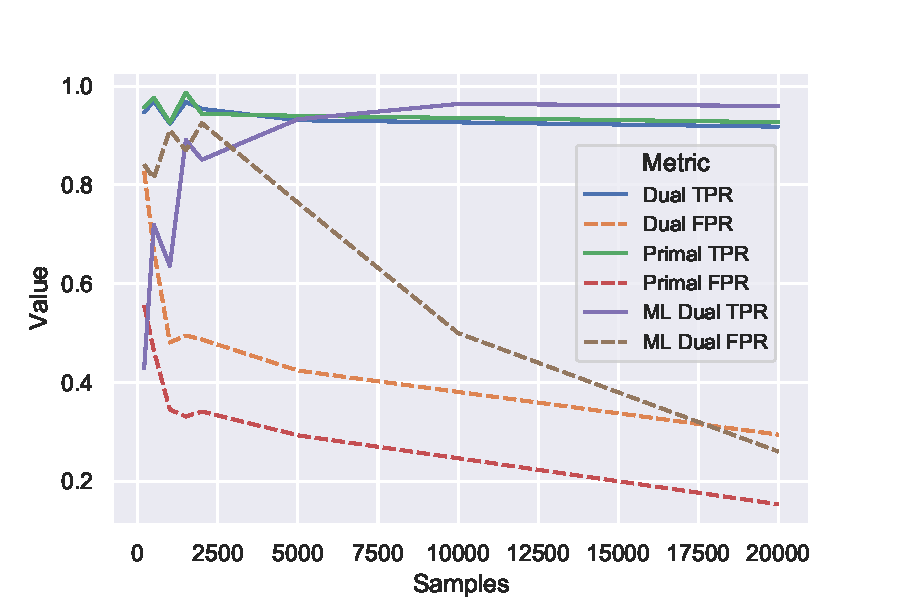
\includegraphics[width=0.5\linewidth]{figures/combined_verma_tests.pdf}
	\caption{A caption to an unrelated (to the text) but interesting figure.}
	\label{fig:validation}
\end{figure}




%%%%%%%%%%%%%%%%%%%%%%%%
% Results
%%%%%%%%%%%%%%%%%%%%%%%%
\section{Results}
\label{sec:results}
Write up and visualize more results here $\dots$


%%%%%%%%%%%%%%%%%%%%%%%%
% Results
%%%%%%%%%%%%%%%%%%%%%%%%
\section{Ablation Study}
\label{sec:ablation}
Perform an ablation study

%%%%%%%%%%%%%%%%%%%%%%%%%
% Discussion + Conclusion
%%%%%%%%%%%%%%%%%%%%%%%%%
\section{Discussion and Conclusion}
\label{sec:discussion}
Provide a discussion on the results of your analysis based on results presented in Section~\ref{sec:results}$\dots$


%%%%%%%%%%%%%%%%%%%%%%%%%
% References
%%%%%%%%%%%%%%%%%%%%%%%%%
\newpage
\bibliography{references}


\end{document}

